%\documentclass[10pt,a4j]{utjarticle}
\documentclass[b5j,twoside,twocolumn]{utarticle}
%\documentclass[b5j,twoside]{utarticle}
%\documentclass[b5j,twoside,twocolumn]{utbook}
\setlength{\columnsep}{2zw}
\usepackage{bxpapersize}
\usepackage{pxrubrica}
\rubysetup{<hj>}
\usepackage{endnotes}
\usepackage{multicol}
\usepackage{plext}
\renewcommand{\theendnote}{[後注\arabic{endnote}]}
\renewcommand{\thefootnote}{\arabic{footnote}}
\usepackage{pxftnright}
\usepackage{fancyhdr}
\setlength{\topmargin}{5mm} % ページ上部余白の設定(182mm x 257mmから計算)。
\addtolength{\topmargin}{-1in} % 初期設定の1インチ分を引いておく。
\setlength{\oddsidemargin}{21mm} % 同、奇数ページ左。
\addtolength{\oddsidemargin}{-1in}
\setlength{\evensidemargin}{17mm} % 同、偶数ページ左。
\addtolength{\evensidemargin}{-1in}
\setlength{\footskip}{-5mm}
%\setlength{\marginparwidth}{23mm}
%\setlength{\marginparsep}{5mm}
\setlength{\textwidth}{225mm} % 文書領域の幅(上下)。縦書と横書でパラメータ(width / height)の向きが変わる。
%\setlength{\textheight}{150mm} % 文書領域の幅(左右)
\makeatletter
\def\@cite#1#2{\rensuji{[{#1\if@tempswa , #2\fi}]}}%%
\def\@biblabel#1{\rensuji{[#1]}}%%%
\makeatother
\usepackage{enumerate}
\usepackage{braket}
\usepackage{url}
\usepackage[dvipdfmx]{graphicx}
\usepackage{float}
\usepackage{amsmath,amssymb}
\newcommand{\relmiddle}[1]{\mathrel{}\middle#1\mathrel{}}
\usepackage{ascmac}
\usepackage{okumacro}
\usepackage{marginnote}
%\usepackage[top=15truemm,bottom=15truemm,left=20truemm,right=20truemm]{geometry}
\usepackage{cleveref}
\usepackage{plext}
\usepackage{pxrubrica}
\usepackage{amsmath}
\usepackage{fancybox}
\usepackage[dvipdfmx]{graphicx}
\usepackage{cancel}
\setcounter{tocdepth}{3}

%\renewcommand{\labelenumi}{(\Alph{enumi})}
\usepackage {scalefnt}
\makeatletter
\@definecounter{yakuchu}
\@addtoreset{yakuchu}{document}% <--- depende on class file
\def\yakuchu{%
\@ifnextchar[\@xfootnote %]
{\stepcounter{yakuchu}%
\protected@xdef\@thefnmark{\theyakuchu}%
\@footnotemark\@footnotetext}}
\def\yakuchutext{%
\@ifnextchar [\@xfootnotenext %]
{\protected@xdef\@thefnmark{\theyakuchu}%
\@footnotetext}}
\def\yakuchumark{%
\@ifnextchar[\@xfootnotemark %]
{\stepcounter{yakuchu}%
\protected@xdef\@thefnmark{\theyakuchu}%
\@footnotemark}}
\makeatother

\usepackage{atbegshi,etoolbox}

\newcounter{newfoot}
\patchcmd{\footnotetext}{\thempfn}{\thenewfoot}{}{}

\newcommand{\evenfootnote}[1]{%
  \ifodd\value{page}%
    \footnotemark%
    \AtBeginShipoutNext{%
      \stepcounter{newfoot}\footnotetext{#1}%
    }%
  \else%
    \stepcounter{newfoot}\footnote{#1}%
  \fi%
}


\pagestyle{fancy}

\title{人形愛のすゝめ}
\author{金重有哉}
\date{\vspace{-5mm}}
\setcounter{page}{107}

\begin{document}
\maketitle

\setlength{\footskip}{-2mm}
\lhead[]{【エッセイ】}
\chead[]{}
\rhead[人形愛のすゝめ]{}
\lfoot[]{\thepage{}}
\cfoot[]{}
\rfoot[\thepage{}]{}

\let\yakuchu=\endnote
\renewcommand{\footnoterule}{\noindent\rule{100mm}{0.3mm}\vskip2mm}
%\tableofcontents
\thispagestyle{fancy}
\section*{人形とはなにか}
あなたが人形と聞いた時に思い浮かべるものはなんでしょうか。西洋のビスクドール、黒髪の日本人形、あるいは藁人形かもしれません。しかし、ここで対象とする人形は人の形に限定されず、テディベアやAIBOなども含みます。人形とは何かの定義に関して、広い定義としては人間が作り出すものは全て人形であるという立場も存在しますが、人間の主観によって生を与えられるものと考えます。


彼らに共通するのは、生きてもいないし死んでもいないということです。生きていないことに関して疑問を持たれる方は少ないかと思われますが、彼らは同様に死んでもいません。その生が客観ではなく人間の主観によって与えられる為、与えられている間仮想的に生きていることになります。


私たちが人間とコミュニケーションを行う際、相手の人間には意識があり、大凡この行動に対してこの反応が返ってくる、と想定することができます。ここで、常識的には自分が存在し、他人も等しく個体として存在しているという認識が生じていると思います。しかし、幼少期はどうでしょうか。自分と他人の区別がつくのは三歳ごろと言われていて、一般的に錯誤問題を解けるようになるのもそのあたりの年齢かと思われます。また、子供の頃ぬいぐるみを抱いて寝ていた人はどうでしょうか。そのぬいぐるみは友達では無かったでしょうか。


人間と人形の差異として、反応が返ってくるかどうか、そしてその反応を想定しているかが重要な点になります。


生きている人間は基本的には話しかけたら返事をするか無視するか気づかないか、いくつかの可能性が考えられます。しかし、ぬいぐるみに話しかけても彼らが気づいてくれることはありません。あるいは内部にセンサを搭載していればそれに応じた反応は返すことはできるかと思います。


しかし、その反応を自分で想像したらどうでしょうか。ぬいぐるみを抱きしめた時、ぬいぐるみはどのように反応するか考えてみましょう。彼らは嫌がりません。そもそも動かないので嫌がらないわけですが、それを嫌がっていないと私たち自身が解釈することができます。そして、その解釈はしばしば自分にとって都合の良い解釈になります。


解釈に関して例を挙げると、ハグビーという抱いて会話する通信メディアが挙げられます。ハグビー自体はあくまで一つの個体として存在せず電話の向こうの誰かの代替でしかないですが、ハグビーを用いて人と会話した際に、相手に対してより良い印象を得られた実験結果があります。ハグビーは人形のようなデザインにおける作り込みはありませんが、足りない部分を人間に補完させることでより良い解釈を促していると捉えることができます。\\


今までの話では、人間がいかに人形を解釈しうるか、という流れの中で人間的なコミュニケーションをとるための方法を紹介しました。しかし、愛するためには人間であること以上に、単に愛を向けるに適切であると思える存在を探すことが重要になります。今多くの人々が人間を愛しているのは慣習的にそれが正しいとされていて、その周辺の存在を考えていないからです。

\section*{一方的な愛の形成}
そもそも愛とは相互に形成されるものなのでしょうか。これに関する議論は様々ですが、人間の外側を考える場合には自分の定義した愛と同じ愛が返ってくることはありません。


一方的な愛の試みの例を紹介として、初音ミクが挙げられます。彼女は生まれの時点で自我を持たず、個体としての初期のインタフェースは音声合成ソフトとパッケージのみでした。彼女はファンによって歌を作られる中でキャラクターが作られ、肉体を持たないながらも歌うアンドロイドとして人格が形成されていきました。印象的なシーンとして、とあるライブで彼女が歌っている途中で機材の不良により一時的にライブが中断されたことがあります。その時観客は機材に向けてではなく、彼女の名前を呼び、彼女に対して声援を送り続けていました。この例は特定の場面に限定されていますが、人格を仮定してそれを愛することが人間以外にも可能であることを示唆していると考えています


人間側の愛とは逆に、人形から人間への愛の例を挙げます。トイ・ストーリーではウッディを始めとしたおもちゃたちが持ち主の見ていないところで動き出します。フィクションなので動き出すわけですが、彼らはそれ自体が動くことで生を持つ他に、現実には持ち主との関係によって生を持つことで、肉体的な生とともに人間によって与えられる生の二重の生を生きています。しかし、彼らは人前で動くことができないので持ち主に愛されることを願い続けるだけです。


これはフィクションですが、制作の側にまわると人形が人間に愛されることを期待する、ということ自体を人間が人形に対して期待している構造が見えてくるわけです。お互いに愛されることが無理だということを理解した上でその愛を求めています。

\section*{おわりに}
愛することに関する議論を行う場合に注意する点として、あくまで愛されることとは別ということです。愛されることは愛することを定義した時点でそれを受けるように定義されるべきで、混同してはいけません。本稿では比較的人間に近い外堀を埋めるような例を紹介しましたが、人間以外のものに対する愛を考え、人間のあるべき姿を探索する可能性を発見できれば、と思います。
\begin{figure}[h]
\centering
\begin{tabular}<y>{c}
\begin{minipage}[c]{0.8\hsize}
\centering
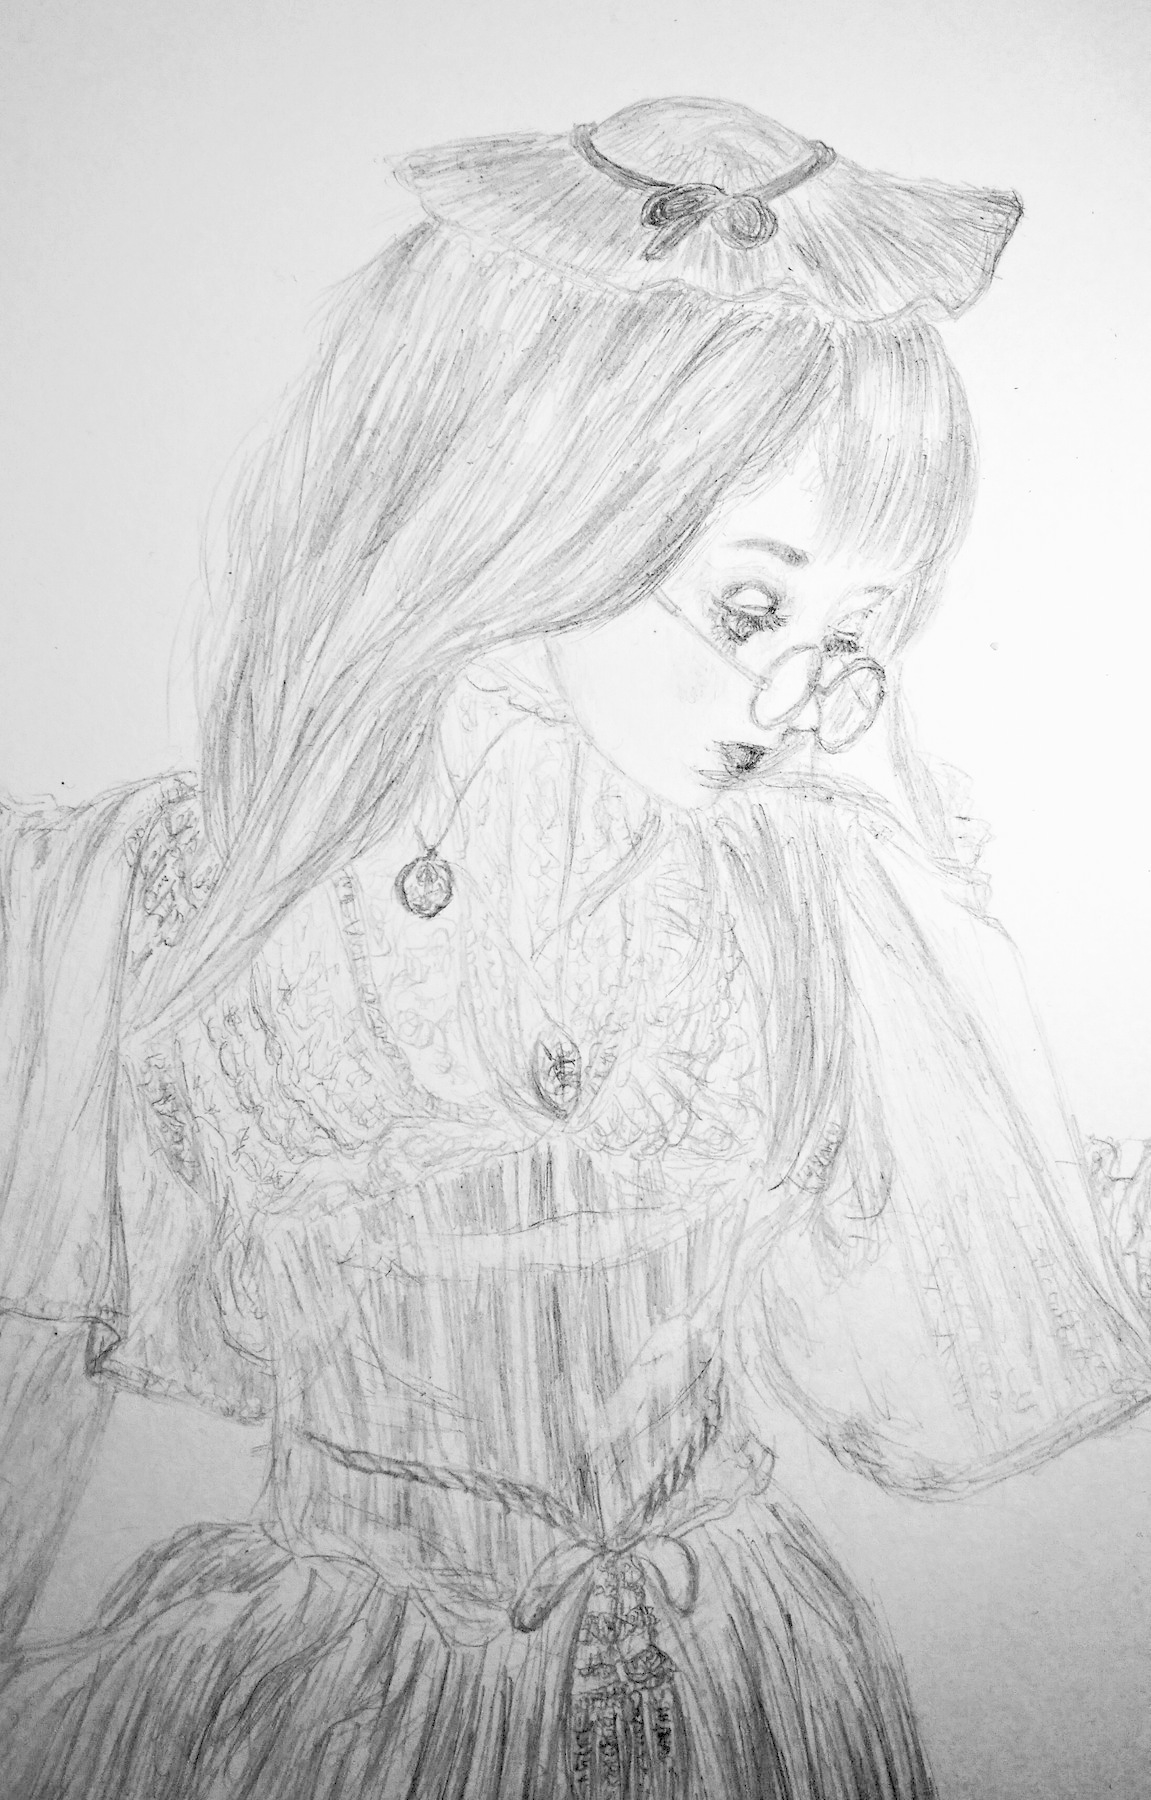
\includegraphics[scale=0.22]{n3I9SWuM}
\caption{筆者の愛}
\end{minipage}
\end{tabular}
\end{figure}

\section*{参考文献}
{\small
\begin{enumerate}
\renewcommand{\labelenumi}{\pbox<y>{[\arabic{enumi}]}}
\item 菊地浩平「人形メディア学講義」河出書房新社 二〇一八
\item 金森修「人形論」平凡社 二〇一八
\item 藤田博史「人形愛の精神分析」青土社 二〇〇六
\item エーリッヒ・フロム、鈴木晶訳『愛するということ 新訳版』紀伊国屋書店 一九九一
\item 中西惇也、桑村海光、港隆史、西尾修一、石黒浩.\pbox<z>{人型対話メディアにおけ}\\ \pbox<z>{る抱擁から生まれる好意.電子情報通信学会 2016, vol.99, no.1, pp.36-44.}
\end{enumerate}
}



\end{document}
